\chapter{Application of \& \dEchorate}\label{ch:dechorateapp}

% \openepigraph{Signal, a function that conveys information about a phenomenon.
% $[\dots]$ Consider an acoustic wave, which can convey acoustic or music information.}{R. Priemer, \textit{Introductory Signal Processing}}

\vspace{-2.5em}
\marginpar{%
    \footnotesize
    \textbf{Keywords:} Early reflection, Speech Enhancement, Beamforming, Room Geometry Estimation, Reflector Estimation.
    \\\textbf{Resources:}
    \begin{itemize}
        \item \href{www.github.com/Chutlhu/dEchorate}{\library{dEchorate} dataset}
        \item \href{www.github.com/Chutlhu/dEchorate}{\library{dEchorate}}
        \item \href{www.github.com/Chutlhu/Risotto}{\library{Risotto}}
        \item \href{www.github.com/Chutlhu/Brioche}{\library{Brioche}}
    \end{itemize}
}
\newthought{Synopsis} \synopsisChDecharateApp



\mynewline
This chapter is a continuation of the~\cref{ch:dechorate} and it is the results of the collaboration with prof. Sharon Gannot and ing. Pinchas Tandeitnik at the Bar'Ilan University, Israel.
The algorithms presented here are straightforward extention of the one available in the literature.
Nevertheless, they are gathered and implemented in the following Python library available online:
\library{dEchorate} related to the \acs{DECHORATE} dataset, \library{Risotto} for \acs{RIR} estimation, \library{Brioche} for echo-aware spatial filtering.
A description of these libraries in reported in the~\cref{ap:code}.

\section{Echo-aware speech enhancement}\label{sec:dechorateapp:se}

\subsection{Literature review}

The knowledge of early echoes should boost audio scene analysis task.
In the previous chapters we showed its application to sound source separation (\cref{ch:separake}) and sound source localization (\cref{ch:mirage}).
However, as discussed in details in~\cref{pt:estimation}, the perfect knowledge of such elements are of difficult estimation.
In this section we investigate this in the context of spatial filtering.
To this end, we compare two types of spatial filters: echo-agnostic and echo-aware beamformers.
Moreover we will evaluated their performances on both synthetic and measured data, both available in the \dEchorate{} dataset (\cref{ch:dechorate}).
As for all the methods presented in this part of the thesis, we assume that echoes are known.
In particular we used the annotation that comes with the considered dataset.
The literature of spatial filtering can be dichotomized in the following two classes.

\newthought{Echo-agnostic beamformers} do not need any echo-estimation step:
they either ignore their contributions, such in the direct-path beamformers ($\DS$)~\citeonly{VanTrees2004Optimum}, nor they consider coupling filters between pairs of microphones, called \ReIRdef/~\citeonly{gannot2001signal}.
In their vanilla form, both the approaches do not the acoustic channel is not computed explicitly.
In case of direct-path beamformer, only the \DOAs/ of the target source is used to build the ideal-path (relative) steering vector.
In order to cope with distortions due to reverberation, external noise or interfering speakers, their statistical description can be included in extended beamformer design, such as the \MVDRtxt/~\citeonly{VanTrees2004Optimum}.
\\The \ReIRs/ have been introduced with the explicit purpose of avoiding the computation of the acoustic channel related to each microphone~\citeonly{gannot2001signal}.
Instead of estimating the dry source signal, they return the reverberant source spatial image at the reference microphone.
Compare to the difficult task of estimating the acoustic channels and the issues of relying on a bad channel estimates, in many practical scenarios this is typically sufficient\sidenote{
    Note that, as opposed to channel estimation, estimating the \ReTF/ is a non-blind problem (See~\cref{sec:processing:rtf}}).
Since then, they have been incorporated in powerful beamforming algorithms\sidenote{A comprehensive review of these methods is available in~\citeonly{gannot2017consolidated}}
In particular, the have been used speech dereverberation and noise reduction both in static~\citeonly{Schwartz2014multi, Kodrasi2017evd}.

\newthought{Echo-aware beamformers} instead model explicitly multipath sound propagation.
They can be seen as \textit{rake receivers}, borrowing the idea from telecommunication where an antenna rakes (\textit{i.e.} combines) coherent signals arriving from different propagation paths.
In particular, they consider ``extended'' steering vectors, whose formulation uses known echoes' delays and attenuations~\citeonly{flanagan1993spatially, Jan1995matched}.
Since then, this approach has been extended in attempt to enhance desired signal in the context of the cocktail party.
For instance, it have been used for interfer and noise suppression in~\citeonly{Dockmanic2015raking} and for noise and reverberation reduction~\citeonly{peled2013linearly, Javed2016spherical, Kowalczyk2019raking}.
In particular, the work~\citeonly{peled2013linearly} estimates the early reflection in the spherical harmonic domain and uses their \DOAs/ to build \ReIR/.
However this approach is not generalizable to all microphone array configuration as they require the deployment of (3D) spherical arrays.
Alternatively, the authors of~\citeonly{dokmanic2015raking}, with its extention to the time-domain~\citeonly{scheibler2015raking}, proposes to modify the original formulation of the \DStxt/ and \MVDRtxt/ beamformer designs to include the knowledge of the echoes as image sources.
While their study is limited to the case of interferer and uncorrelated noise reduction, while the later reverberation reduction is not considered.
As opposed to, the recent work of~\citeonly{Kowalczyk2019raking} address the problem of enhancing a single target speech source affected simultaneously by both noise and late reverberant.

\mynewline
In this work, we compare the beamformer designs proposed in~\citeonly{Kowalczyk2019raking} for noise and late reverberation reduction.
Nevertheless, we took a different point of view: we investigate the influence of correctly estimated echoes when using either synthetic nor measured impulse response.

\subsection{Background in spatial filtering}
Given the narrowband \STFT/ signal model presented is~\cref{subsec:processing:model:stft}, the signals captured by $\numMics$ microphone listening to a single sound source ($\numSrcs=1$) in a noisy reverberant room, reads:
\begin{equation}
    \MICS[k,l] = \FLTS[k] \SRC[k, l]+ \NSES[k,l]
    ,
\end{equation}
where $\MICS[k,l], \FLTS[k,l], \NSES[k,n] \in \bbC^{\numMics}$.
Note than, since only one sound source is considered ($\numSrcs=1$), the mixing matrix $\FLTS[k]$ reduces to a vector and $\SRC[k,l] \in \bbC$ to a complex scalar.
\\The filters vector can be decomposed in order to highlight the sound propagation components, that is,
\begin{equation}
    \FLTS[k] = \kbracket{\FLT^{\mathtt{dp}}_{\idxMic}[k]+ \FLT^{\mathtt{ee}}_{\idxMic}[k] + \FLT^{\mathtt{lr}}_{\idxMic}[k] }_\idxMic
\end{equation}
where the summands correspond to the direct-path ($\mathtt{dp}$), early echoes ($\mathtt{ee}$) and late reverberation ($\mathtt{lr}$), respectively.
The early part of the \RIR/ associated to the $i$-th channel follows the echo model, that is,
\begin{equation}
    \FLT^{\mathtt{dp}}_{\idxMic}[k]+ \FLT^{\mathtt{ee}}_{\idxMic}[k] = \sum_{\idxEch=0}^{\numEchs} \alpha_{\idxMic}^{(r)} \cste^{-\csti 2 \pi f_k \tau_i^{(r)}}
    ,
\end{equation}
being the $\idxEch=0$ the index of the direct propagation.
Hereafter, for the sake of clarity, we omit the dependency on the discrete time-frequency bin $[k,l]$

\mynewline
Given the above decomposition of the \RIRs/, by the associativity of the multiplication, the vector $\MICS$ can be expressed accordingly as:
\begin{equation}\label{eq:dechorateapp:mics}
    \MICS = \MICS^{\mathtt{dp}} + \MICS^{\mathtt{ee}} + \MICS^{\mathtt{lr}} + \NSES[k,n]
    ,
\end{equation}

\mynewline
In the context of echo-aware spatial filtering, the source signal of interest include both the direct path and the $\numEchs$ early reflection, as done in~\citeonly{dokmanic2015raking,Kowalczyk2019raking}
This assumption is motivated by pyschoacoustics studies as discussed in~\cref{ch:acoustics:sec:perception}.
In particular, they showed the first early echoes contributes to increase speech intelligibility, as they are fully integrated in the direct direct sound increasing its perceived intensity.
Based on this, we define as the signal of interest the following component
\begin{equation}
    \MICS_s = \MICS^{\mathtt{dp}} + \MICS^{\mathtt{ee}}
\end{equation}

\mynewline
Noise and the late reverberation are typically describe as random process.
Therefore, it is common to express the microphone signal model of~\cref{eq:dechorateapp:mics} from a statistical point of view.
To this end, \xPSD/ matrix of the microphone signal, $\xpsd_{\mic} = \bbE\kbrace{\mic \khermitian{\mic}} \in \bbC^{\numMics \times \numMics}$ reads
\begin{equation}
    \xpsd_{\mic} = \FLTS \xpsd_{\src} \khermitian{\FLTS} + \xpsd^{\mathtt{lr}}_{\mic} + \xpsd_{\nse}
    ,
\end{equation}
where $\bbE[\cdot]$ denotes the expectation operator.
Here $\xpsd^{\mathtt{lr}}_{\mic}$ and $\xpsd_{\nse}$ denotes the \xPSD/ of the late reverberation and noise, respectively.
Since we assume that all the spatial information is expressed by the filters $\FLTSS$, the source \xPSD/ matrix $\xpsd_\src$ is assumed here to be diagonal
\begin{equation}
    \xpsd_\src = \sigma_\src^2 \bfI
    ,
\end{equation}
where $\bfI$ is the identity matrix of dimension $\numMics \times \numMics$ and $\sigma_\src^2 = \bbE\kbrace{\powerOf{\SRC}}$.

\newthought{The late reverberation} \xPSD/ matrix can be estimated using the time-invariant spatial coherent matrix model proposed in~\citeonly{kuster2012objective}, based a diffuse sound field model~\citeonly{kuttruff2009room}.
\begin{equation}
    \xpsd^{\mathtt{lr}}_{\mic} = \sigma_{lr}^2\mathbf{\Gamma}
    ,
\end{equation}
where $\sigma_{lr}^2$ denotes the power of the late reverberation and $\mathbf{\Gamma}$ is the $\numMics \times \numMics$ spatial coherence matrix, which is available in closed-form\sidenote{
    \footnotesize
    Given the distance $\distMicMic_{ii'}$ between to microphone $i$ and $i'$, the interchannel coherence function in the continuous-frequency domain writes
    \begin{equation*}
        \tilde{\gamma}_{ii'}(f) = \frac{\sin(2 \pi \distMicMic_{ii'} / \speedOfSound)}
                                        {2 \pi \distMicMic_{ii'} / \speedOfSound}.
    \end{equation*}
    Then, the matrix $\mathbf{\Gamma}$ is built by computing the $\tilde{\gamma}$ for all the pairs of channel on a discrete set of frequencies.
}.
This approach have been found successful in many dereverberation application~\citeonly{dereverberation2010pa, cauchi2014joint, tammen2018iterative}

\newthought{The additive noise} \xPSD/ matrix can be easily estimated from the microphone recording using non-speech segment.
In blind setting, this would require the usage of a voice activity detector.
Alternatively, the noise component can be modeled as a random process whose spatial covariance matrix can be estimated with advance techniques.


\subsection{Beamforming designs}
In the \STFT/ domain, a beamformer forms a linear combination of the microphone channels to yield the desired output $U[k,l]$.
That is,
\begin{equation*}
    U[k,l] = \ktranspose{\bfW} \MICS = \ktranspose{\bfW} \FLTSS \SRC + \ktranspose{\bfW} \NSES,
\end{equation*}
where the vector $\ktranspose{\bfW} \in \bbC^{\numMics}$ contains the beamformer weights.
\\This weights can be computed in order to optimize design criterions.
Common examples of beamformers are the \DStxt/, the \MVDRtxt/, the \MaxSNRtxt/, the \MaxSINRtxt/, and the \LCMVtxt/.

In the context of a consolidated spatial filtering framework~\citeonly{gannot2017consolidated}, we can identified following levels of complexity in beamformer design:
\begin{enumerate}
    \item \DStxt/ only the steering vectors towards a defined direct is considered.
    \item \MVDRtxt/
    \item \LCMVtxt/
\end{enumerate}


\newthought{The Delay-and-Sum} is the simplest and ofter quite effective beamformer.
In its vanilla version, the \DS/ is designed to only compensate the propagation delay from the source to the microphones assuming ideal propagation path.
Assuming the far field scenario and $i=0$ being the reference microphone, this is typically achieved using the direct-path steering vector $\bfD$ defined in~\cref{eq:processing:relativesteering}, that is,
\begin{equation}
    \hat{\bsD}_{j}[k] = \klist{
                         1,
                         \cste^{-\csti 2 \pi f_k \tau_{i+1}^{(r)} / \speedOfSound},
                         \ldots,
                         \cste^{-\csti 2 \pi f_k \tau_{i}^{(r)} / \speedOfSound}
                    }
\end{equation}

Therefore,

\begin{equation}
    \bsW_{\mathtt{dp}} = \frac{\bsD}{\kvvbar{\bsD}}
\end{equation}

\newthought{MVDR}  design optimize the following criterion
\begin{equation}
    \bsW_{\MVDR} = \kargmin_{\bsW} \kbrace{ \khermitian{\bsW} \xpsd_{\NSES} \bsW\;\text{s.t.}\;\khermitian{\bsW} \bsD}
\end{equation}

\newthought{RTF-MVDR}
In this work, generalized eigenvector decomposition (GEVD) was used for the RTFs estimation~\citeonly{doclo2003robust}.

\newthought{Rake-MVDR}

\newthought{MVDR with late reveberation}

\subsection{Experimental evaluation}
The performances of the different designs are compared for enhancing a target speech in 5-channel mixture (that is, one linear array used in the \dEchorate{} dataset).
In particular, they are tested in scenarios featuring high reverberation and diffuse babble noise, opportunely scaled to given pre-defined signal-to-noise ratio ($\SNR \in \kbrace{0, 10, 20}$).
Using the \dEchorate{} data, we considered the room configuration $\mathtt{011111}$ ($\RT \approx 600 $ ms) and all the possible combinations of target/array's positions.
Both real and matching synthetic \RIRs/ are used which are then convolved with anechoic speech from the \WSJ/ corpus and corrupted by recorded diffuse noise.

\mynewline
The evaluation is conducted similarly to the one in~\citeonly{Kowalczyk2019raking}.
Therefore, we considered the following metrics:


\newthought{The Signal-to-Noise-plus-Reverberation Improvement} (\DSNRR) in [dB] computed as difference between the input ($\mathtt{SNRR}_\mathtt{i}$) at the reference microphone and the $\mathtt{SNRR}_\mathtt{o}$ at the filter output.
    \begin{equation}
        \begin{aligned}
            \mathtt{SNRR}_\mathtt{i} &=\\
            \mathtt{SNRR}_\mathtt{o}&=\\
            \DSNRR &= \mathtt{SNRR}_\mathtt{o} - \mathtt{SNRR}_\mathtt{i}
        \end{aligned}
    \end{equation}

\newthought{The Speech-to-Reverberation-Energy-Modulation Ratio Improvement} (\DSRMR)\citeonly{falk2010non} as measure of dereverberation.
\begin{itemize}
    \item proposed in~\citeonly{falk2010non}
    \item Cochlear implant preprocessing: The SRMR is obtained by first applying a 23-channel gammatone filterbank to the time domain signal.
    \item A Hilbert transform captures the envelope of the output of each filter, and thus the temporal dynamics information.
    \item These signals are then transformed into the STFT domain to obtain an 8 band modulation spectrum segmented into frames.
    \item The SRMR is then obtained by comparing the energy in the different bands of the modulation spectrum
    \item Lastly, the output value is computed as the ratio of the average modulation energy content available in the first four modulation bands (from 3 Hz up to 15 Hz (20 Hz) for CI, thus consistent with clean speech modulation content [16])
         to the average modulation energy content available in the higher frequency modulation bands (circa 20–160 Hz for the SRMR, 15–82 Hz for the CI-adapted version).
\end{itemize}

\newthought{The Perceptual Evalutation of Speech Quality} is evaluated using the PESQ score.
\begin{itemize}
    \item presented in~\citeonly{rix2001perceptual}
    \item a measure assumed to cover several speech degradation and distortion was promoted in the ITU-T recommendation P.862 [ITU-T 2001]
    \item This metric named “Perceptual Evaluation of Speech Quality” (PESQ) is for now considered as one of the most reliable metric to predict the overall speech quality
    \item PESQ was first designed to account mainly for network or telecommunication distortion
    \item the signals are equalized following the typical frequency response of a telephone
    \item Practically, after applying an auditory model to the signals (based on a Bark frequency scale) the loudness spectra are estimated.
    \item From the loudness spectra differences (disturbance), the wideband PESQ predicts a Mean Opinion Score (MOS) as it could be retrieved from genuine listening tests.
    \item Mean opinion score (MOS) is a measure used in the domain of Quality of Experience and telecommunications engineering, representing overall quality of a stimulus or system. It is the arithmetic mean over all individual "values on a predefined scale that a subject assigns to his opinion of the performance of a system quality".
    \item The MOS is expressed as a single rational number, typically in the range 1 to 5
    \item PESQ output scores range from 1 (bad) to 5 (excellent).
\end{itemize}

As target signal, the clean signal convolved with the early part of the RIR (up to the $R$-th echo) is considered.

Numerical results are reported in Figure~\ref{fig:dechorateapp:se:results}.
\begin{figure}[h]
    \begin{fullwidth}
        \centering
        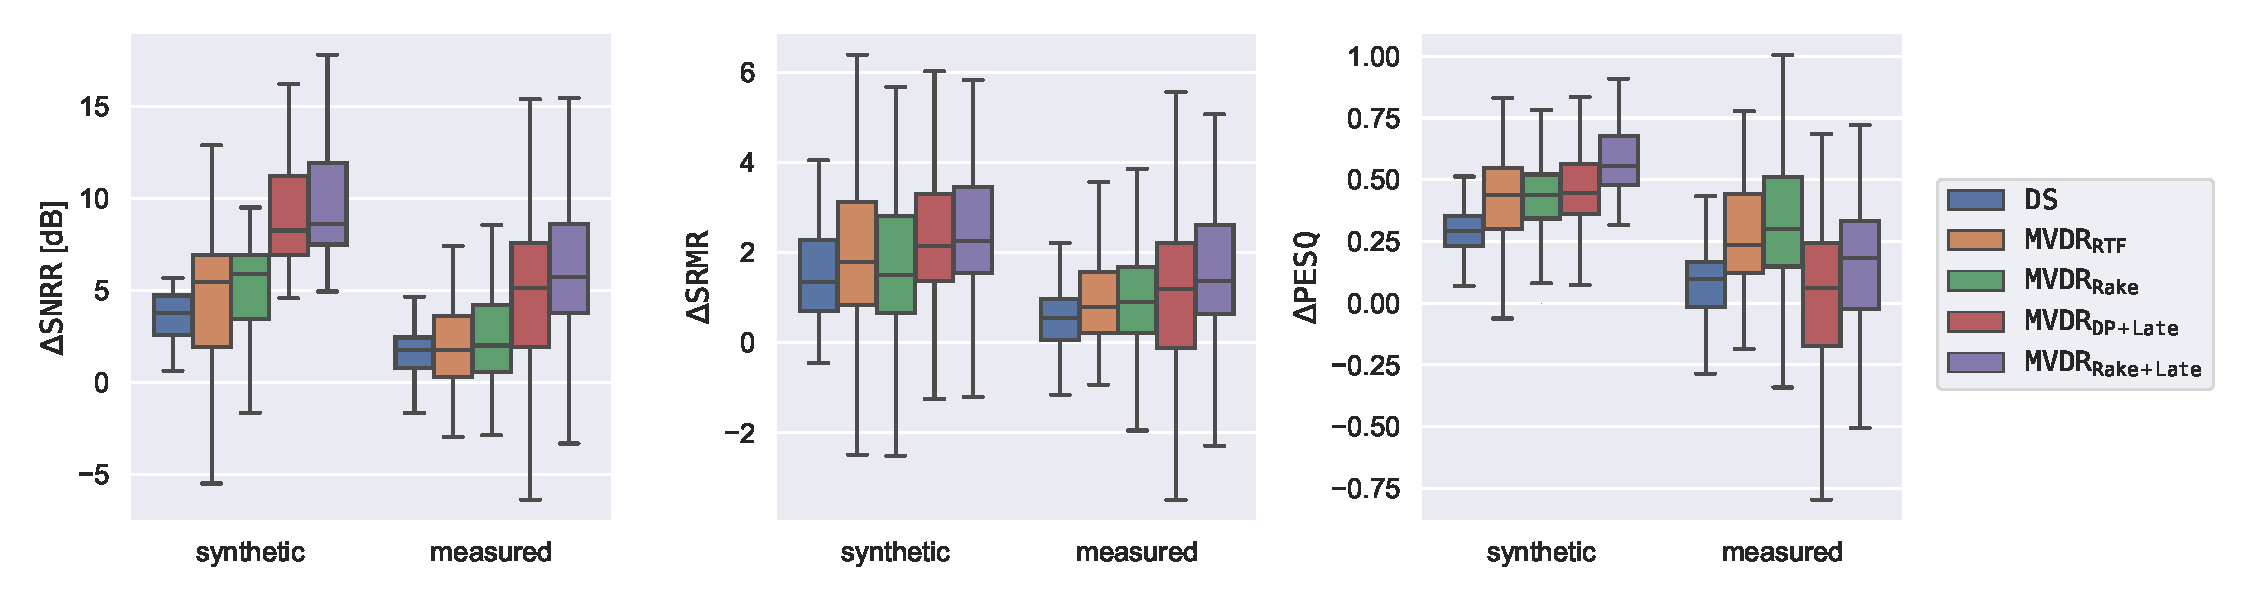
\includegraphics[trim={0 10 10 0},clip,width=\linewidth]{figures/dechorate/kowalkzy_results_boxplot.pdf}
        \caption{
        Comparison of echo-aware beamforming for the room configuration $\mathtt{011111}$ ($\RT \approx 600 $ ms) on measured and synthetic data  for all combinations of source-array positions in the \dEchorate{} dataset.}
        \label{fig:dechorateapp:se:results}
    \end{fullwidth}
\end{figure}
The simple $\DS$ beamformer is outperformed by the other filters, since more information is used to reduce noise and late reverberation.
When using synthetic data, the know echoes perfectly match numerically the components in the simulated RIRs. In this ideal scenario, one can see that the more information used the better the performances: RTF- and Rake- beamformers outperform the simple $\DS$ design; and including the late reverberation statistics boosts considerably all the performances.
Interestingly RTF-based design performs similarly to the Rake-one. This can be explained by the fact that GEVD method tends to robustly consider the stronger and more stable components of the RTFs, which in reverberant and noisy static scenario's are similar to the earlier portion of the RIRs.
\\When it comes to measured RIRs, the little errors in echo estimation, due to calibration mismatch, lead to a drop in the performances. This is even more clear when considering the $\dPESQ$ metrics, as it accounts also for artifacts. Here the echo-agnostic $\MVDR_\mathtt{RTF}$ outperform the other methods.

yup. And it looks like for SNRR/synthetic, Rake+Late would have a slight edge in terms of mean over the others. In general it looks like Rake+Late has more variance than RTF+Late, suggesting that in some situations it performs better, while in other it performs less well. Would be of course interesting to know what influences that exactly

\section{Room Geometry Estimation}\label{sec:dechorateapp:rooge}

The shape of a convex room can be estimated knowing the positions of first-order image sources.
This task is known as \RooGE/ or reflection estimation.
Several methods have been proposed which take into account different levels of prior information and noise and they are briefly discussed in the context of echo labeling in~\cref{subsec:estimation:active_rir}\sidenote{
    This methods have been recently review in \citeonly{remaggi2016acoustic, Crocco2018room}.
}.
Nonetheless, when the echoes' \TOAs/ and their labeling are known for 4 non-coplanar microphones, one can perform this task using simple geometrical reasoning as in \citeonly{Dokmanic2013acoustic}.
In fact, the 3D coordinates of each image source can be retrieved solving a \textit{multilateration} problem \citeonly{Beck2008ExactProblems} and the position and orientation of each wall can be easily derived from the \ISM/ equations as the plane bisecting the line joining the real source position and the position of its corresponding image (see Figure~\ref{fig:dechorateapp:wall_rec}).

\subsection{Using the \dEchorate{} dataset}
In \dEchorate{} the annotation of all the first order images for all the sound sources are available.
Table~\ref{tab:res_rooge} shows the results of the estimation of the wall positions in terms of distance error (in centimeters) and surface orientation error (in degrees) using the four direct sources and all the 30 microphones, namely the 6 arrays).
The room facets are estimated using each of the source as a probe. Despite few outliers, the majority of the facets are estimated correctly in terms of their placement and orientation with respect to the coordinate system computed in Section~\ref{sec:annotation}: for instance, for the source $\#4$, all 6 surfaces were localized with less than $6$ cm and $\ang{2.5}$ errors. Small errors are due to concurrency of multiple factors, such as tiny offsets in the annotation and the ideal shoebox approximation. In the real recording room, some gaps were present between revolving panels in the walls. In addition it is possible that for some source-receiver pairs the far-field assumption is not verified, causing the inaccuracy of \textit{reverting} the ISM. Finally, the 2 outliers for the source $\#3$ are due to a wrong annotation caused by source directivity and mis-classification. When a wall is ``behind'' the source, the energy of the related $1^\text{st}$ reflection is very small and might not appear in the RIRs. This happened for the eastern wall and a second order image was taken instead. Secondly, the contribution of multiple reflections arriving at the same time can results in large late spikes in estimated RIRs. This effect is particularly amplified when the microphone and loudspeakers exhibit long impulse responses. As a consequence, some spikes can be miss-classified. This happened for the southern-wall were again a second-order image was taken instead. Nevertheless, this second type of errors can be manually corrected and the annotations updated.

\begin{figure}[t]
    \begin{fullwidth}
    \centering
    \subfloat[image][Source images estimation]{
    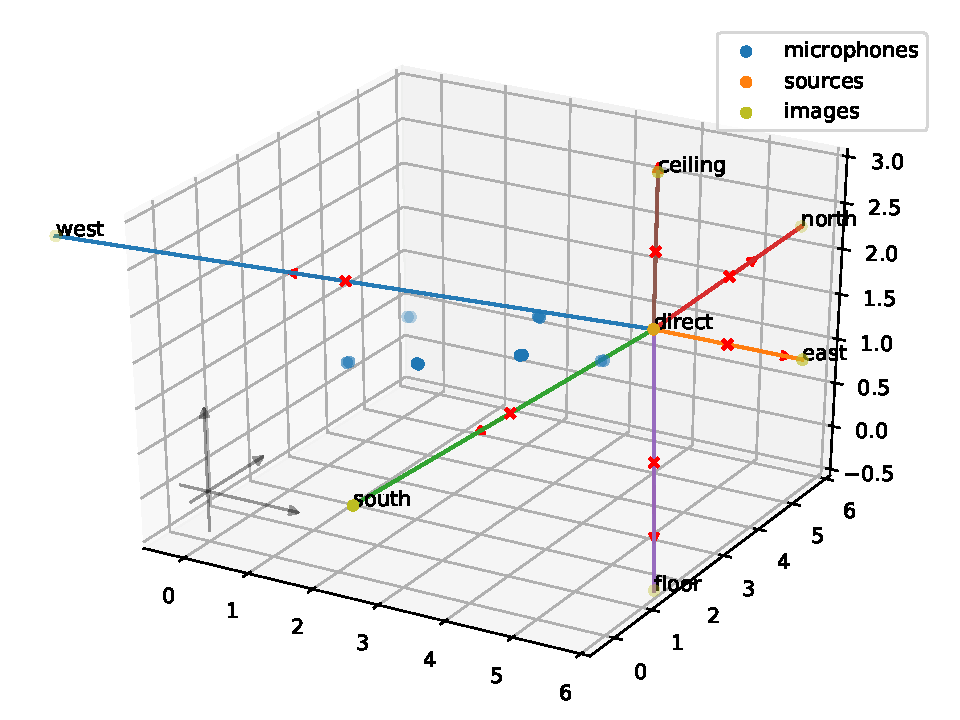
\includegraphics[width=0.48\textwidth]{figures/dechorate/estimated_image}
        \label{fig:dechorateapp:image}
    }
    \hfill
    \subfloat[reflector][Reflector estimation]{
        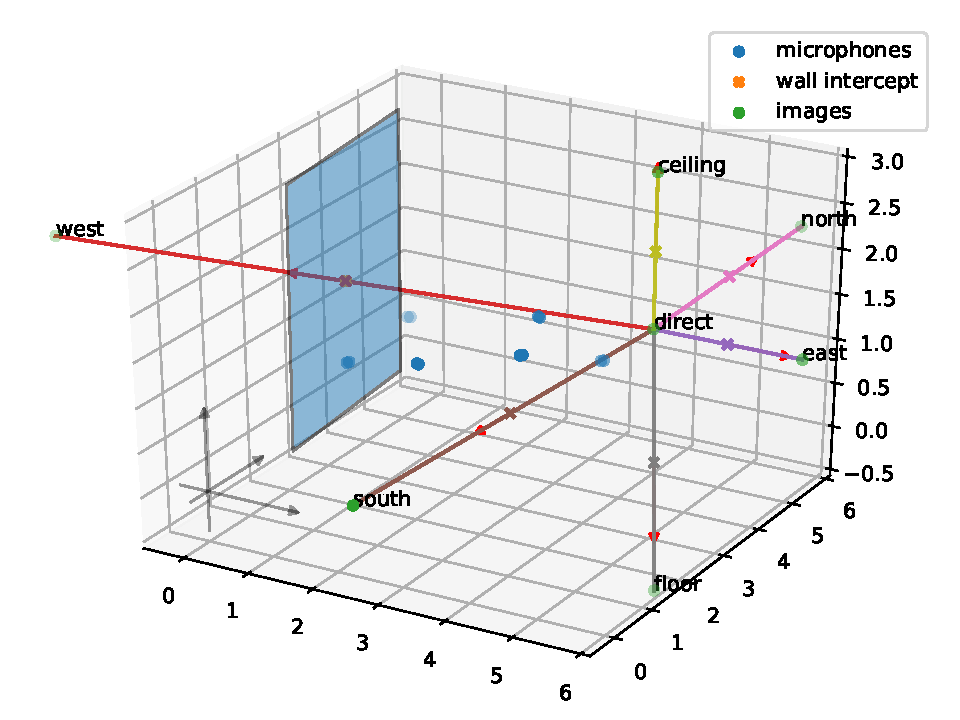
\includegraphics[width=0.48\textwidth]{figures/dechorate/estimated_reflector}
        \label{fig:dechorateapp:reflector}
    }
    \caption{Images source estimation (right) and corresponding reflector estimation (left) for one of the sound sources in the dataset.}
    \label{fig:dechorateapp:wall_rec}
    \end{fullwidth}
\end{figure}

% \begin{figure}

%         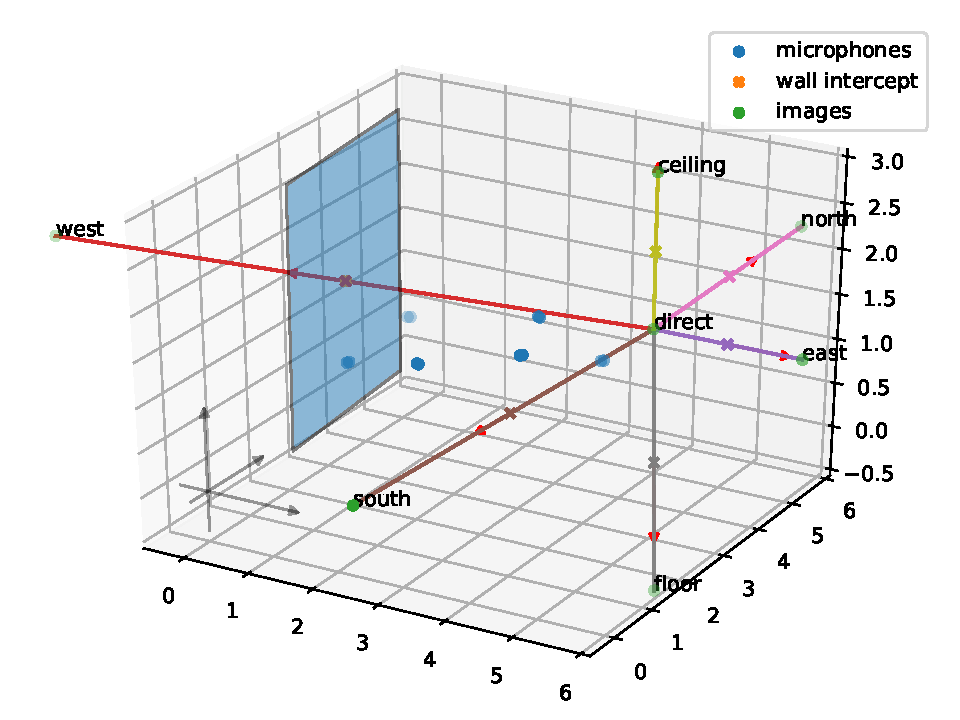
\includegraphics[width=\linewidth]{figures/dechorate/estimated_reflector}

%     \caption{Images source estimation and reflector estimation for one of the sound sources in the dataset.}
%     \label{fig:dechorateapp:wall_rec}
% \end{figure}

\begin{table}[h!]
    \begin{sidecaption}[]{
        Distance errors (DE) in centimeters and angular errors (AE) in degrees between ground truth and estimated room sides using each of the sound source ($\#1$ to $\#4$) as a probe. For each wall, bold font is used in correspondence with the sources yielding the best DE and AE; while, the italic font highlight the outliers, if present.
        }[tab:res_rooge]
    \centering
    \small
    \begin{tabular}{c|cc|cc|cc|cc}
\toprule
source id &	1	& &	2	& &	3	& &	4 &	\\
wall &	DE&	AE&	DE&	AE&	DE&	AE&	DE&	AE\\
\hline
west &	0.74	& $\ang{8.99}$      & 4.59	& $\ang{8.32}$  & 5.89	& $\ang{5.75}$	& $\mathbf{0.05}$    & $\mathbf{\ang{2.40}}$\\
east &	$\mathbf{0.81}$	& $\mathbf{\ang{0.08}}$      & 0.9	& $\ang{0.50}$	&$\mathit{69.51}$	& $\mathit{\ang{55.70}}$	& 0.31    & $\ang{0.21}$\\
south&	3.94	&$\ang{16.08}$      & $\mathbf{0.18}$	& $\ang{1.77}$	&$\mathit{14.37}$ & $\mathit{\ang{18.55}}$	& 0.82    & $\mathbf{\ang{1.65}}$\\
north&	1.34	& $\ang{0.76}$	    & 1.40	& $\ang{8.94}$	& $\mathbf{0.63}$	& $\mathbf{\ang{0.17}}$	& 2.08    & $\ang{1.38}$\\
floor&	$\mathbf{5.19}$	& $\mathbf{\ang{1.76}}$	    & 7.27	& $\ang{2.66}$	& 7.11	& $\ang{2.02}$	& 5.22    & $\ang{1.90}$\\
ceiling&1.16	& $\ang{0.28}$	    & 0.67	& $\ang{0.76}$	& $\mathbf{0.24}$	& $\ang{1.16}$	& $0.48$    & $\mathbf{\ang{0.26}}$\\

\bottomrule
\end{tabular}

    \end{sidecaption}
\end{table}

\section{Conclusions and Perspectives}\label{sec:dechorateapp:conclusion}

This paper introduced a new database of room impulse responses featuring accurate annotation of early echoes and microphone positions. These data can be used to test methods in the room geometry estimation pipeline and in echo-aware audio signal processing. In particular, robustness of these methods can be validated against different levels of $\RT$, SNR or even early echo density.